\documentclass[a4paper]{article}

\usepackage[english]{babel}
\usepackage[utf8]{inputenc}
\usepackage{amsmath}
\usepackage{listings}
\usepackage{color}
\usepackage{hyperref}
\usepackage{float}
\usepackage{graphicx}
\graphicspath{{../pics/}}

\title{Machine Learning (course 1DT071)
Uppsala University – Spring 2015
Report for Assignment 4 by group 6}

\author{Ludvig Sundstr\"{o}m and John Shaw}
\date{\today}

\begin{document}

\maketitle

\section*{Task 1: Genetic Algorithms}

\subsection*{Question 1} 

\emph{Think about what each of the genetic operators means for this
simplistic genome. Geometrically speaking, what would a 1-point crossover look like in this case? What about mutation?}

\textbf{Answer:} When considering the selection, a good fitness function would be to max the radius to the closest star. Ranking would then be the different coordinates sorted from the largest to the smallest radius and we could select an individual with a probability weighted on the rank. 

For reproduction we would just select one individual and copy it to the population.
% (0704) (1513) = (1504) (0713) = 0703 1514 = 0513 1704

For recombination we would select two individuals and perform a crossover. A 1-point selection would geometrically have a few different outcomes depending on were the crossover is performed and how the genome is encoded. The most simple representation would be that the $x_i$ and $y_i$ coordinate of the parent $i$ would be crossed over with the second parent $j$'s coordinates. This would result geometrically with the new individual(s) becoming align with one parent on the x-axis and the other parent on the y-axis. 

We can however imagine more complex representations of the genome that would create more complex crossovers.

A restriction could be that we are not allowed to recombine to a new individual located outside the grid, avoiding memory issues.

Mutation would be to select an individual and introducing some noise into its coordinates. This would produce a new individual that would be more or less a random coordinate but biased to keep many similarities with the original parent. This should be restricted to only produce coordinates within our grid. 

\subsection*{Question 2}
\emph{Would you expect more improvement in this problem to result
from crossovers or mutations? Why? Is that what you would normally expect?}

\textbf{Answer:} Depending on the way we define the crossover it could be hard to cover all the search space with only the crossover operator. The data is scattered randomly in the search space and each individual doesn't contain useful information encoded in its genome that future generations can benefit from. With this crossover implementation we think mutation does us more good since it's similar to a random search. 

\begin{figure}[H] %float here
	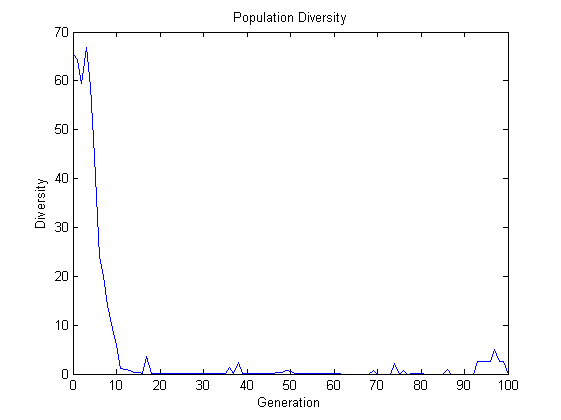
\includegraphics[scale=0.7]{populationDiversityStars.png}
	\caption{\label{fig:plot1Diversity}\textbf{Plot 1} The diversity of the population of coordinates.}
\end{figure}

\subsection*{Question 3}
\emph{What are the possible sources of population diversity when using
genetic algorithms? How do are those sources of diversity reflected in the shape of the diversity curve in your plot?}

\textbf{Answer:} 
Firstly the population diversity can be initialised by random starting positions of the nodes. Secondly crossover and mutation increases the diversity and the peaks in our graph are when the crossover or mutation have lead us to a better solution, increasing the diversity of the general population. 

\subsection*{Question 4}
\emph{Why is population diversity important?}

\textbf{Answer:} Without diversity we can't use the differences of the genomes as much as if we have a lot of diversity. So a good diversity in the start help us not get stuck at a maxima/minima as much as a bad diversity would since the diversity would allow us to faster try other solutions.

\subsection*{Question 5}
\emph{What's the difference between rank and proportional selection?
Why does that make rank based selection better at avoiding premature convergence?}

\textbf{Answer:} In proportional selection the probability of getting selected is directly dependent on the fitness of that individual. In ranked based selection we use the rank-order of the fitness among the individuals to determine the probability, not relying on absolute fitness values. Selection with ranked selection is therefore independent of the actual fitness values and the best individual will not dominate the selection process. %TODO reference to the book.

\begin{figure}[H] %float here
	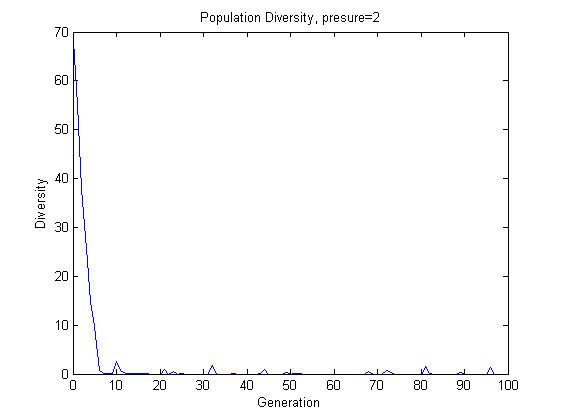
\includegraphics[scale=0.7]{divPress2.png}
	\caption{\label{fig:plot2Diversity2}\textbf{Plot 2} The diversity of the population of coordinates using ranked based selection with a pressure value of 2.}
\end{figure}
\begin{figure}[H] %float here
	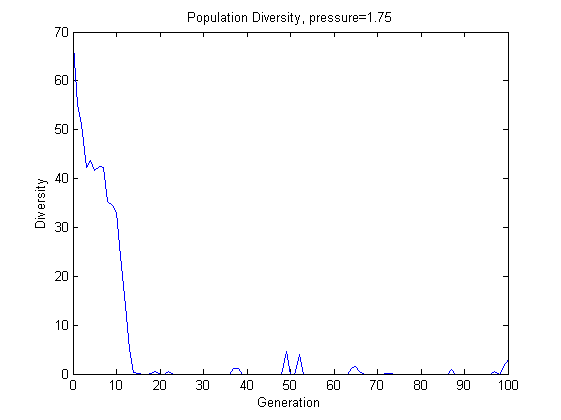
\includegraphics[scale=0.7]{divPress175.png}
	\caption{\label{fig:plot2Diversity175}\textbf{Plot 2} The diversity of the population of coordinates using ranked based selection with a pressure value of 1.75.}
\end{figure}
\begin{figure}[H] %float here
	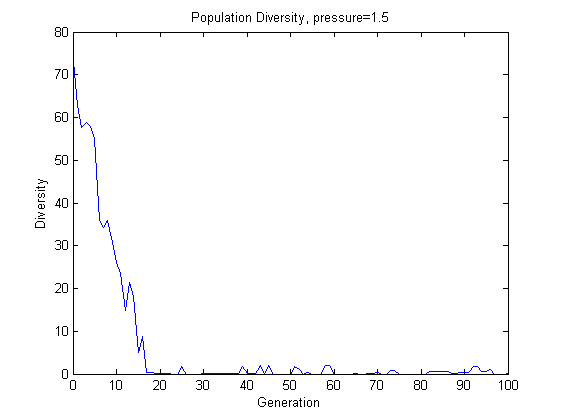
\includegraphics[scale=0.7]{divPress15.png}
	\caption{\label{fig:plot2Diversity15}\textbf{Plot 2} The diversity of the population of coordinates using ranked based selection with a pressure value of 1.5.}
\end{figure}
\begin{figure}[H] %float here
	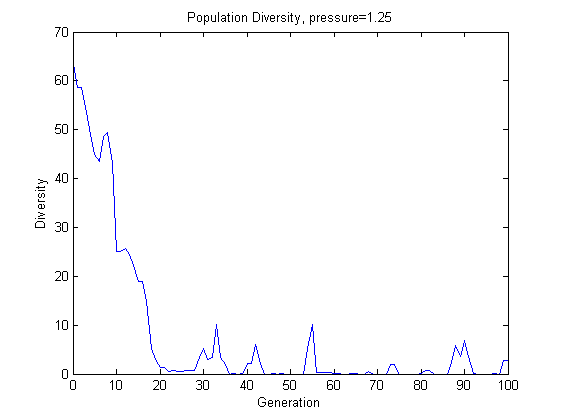
\includegraphics[scale=0.7]{divPress125.png}
	\caption{\label{fig:plot2Diversity125}\textbf{Plot 2} The diversity of the population of coordinates using ranked based selection with a pressure value of 1.25.}
\end{figure}
\begin{figure}[H] %float here
	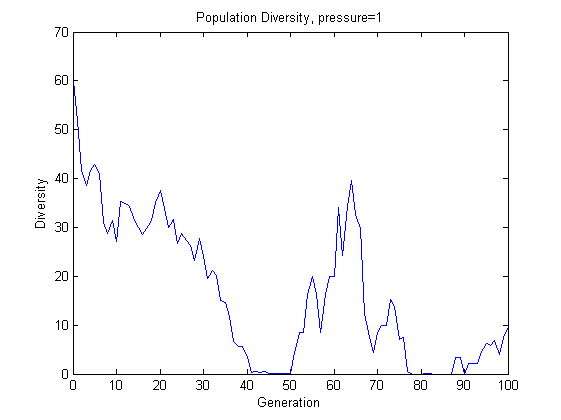
\includegraphics[scale=0.7]{divPress1.png}
	\caption{\label{fig:plot2Diversity1}\textbf{Plot 2} The diversity of the population of coordinates using ranked based selection with a pressure value of 1.}
\end{figure}

\subsection*{Question 6} \emph{What selection pressure resulted in the most
    promising looking diversity curve? Run the algorithm a few more times using
that pressure setting. What was the best fitness value and position you were
able to locate?}

\textbf{Answer:} We think that a pressure of 1.5 looks most promising as seen
in \ref{fig:plot2Diversity15}. Another good candidate is the pressure value of
1.25 \ref{fig:plot2Diversity125}. The big question here is what we consider the
problem to be. Are we looking for the optimal solution or just a good solution?
Another consideration is how much computational time do we have? 

A steep diversity curve as in \ref{fig:plot2Diversity2} leads to a fast
convergence which most likely means it takes the first good enough solution and
optimize for that one. A less steep one means we are considering more less fit
nodes for a longer time, giving us more time to search the space for a better
solution and thus increasing the probability of eventually the globally optimal
solution.

An argument why we like the 1.25 solution is that it still contains some spikes
after the first steep decent of the slope. This suggest that it's still
searching quite a lot for better solutions and thus giving it more generations
to run means it could eventually find better solutions.

%fitness 3.4192 generation 2 crossover
%fitness 3.6057 gen 74 via mutation
%fitness 3.2968 gen 65 via mutation
%fitness 3.1721 gen 83 via mutation
%fitness 3.5711 gen 81 via mutation
%ingen elitism
%gen 27 via mutation
%gen 62 via mutation
%gen 78 via mutation
%gen 19 via mutation
%gen 4 via crossover

%Insert plot 3
\begin{figure}[H] %float here
	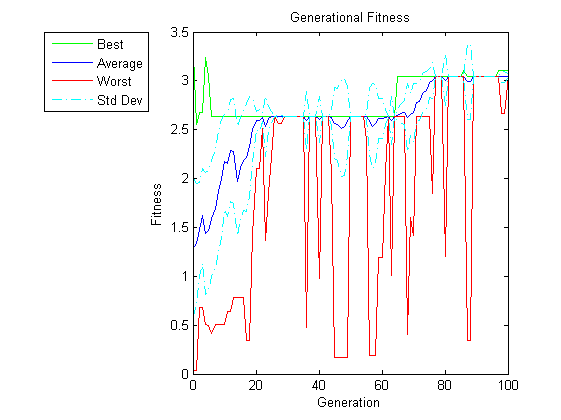
\includegraphics[scale=0.7]{fitness-non-elitist.png}
	\caption{\label{fig:plot3nonelitist}\textbf{Plot 3} A fitness plot without elitist. }
\end{figure}
\begin{figure}[H] %float here
	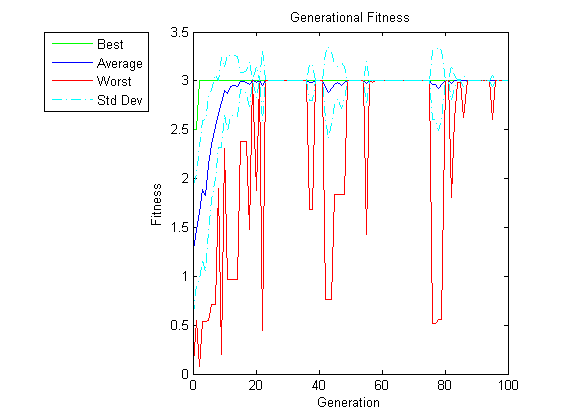
\includegraphics[scale=0.7]{fitness-elitist.png}
	\caption{\label{fig:plot3elitist}\textbf{Plot 3} A fitness plot with elitist. }
\end{figure}


\subsection*{Question 7}
\emph{What affect does an elitist strategy have on the progress of fitness values?}

 \textbf{Answer: } The best fitness value cannot decrease with an elitist strategy. The average fitness is increased more steeply with an elitism strategy and faster catches up with the best value. 

\begin{table}[h]
\begin{tabular}{|l|l|l|l|}
\hline
\multicolumn{2}{|c|}{With Elitist} & \multicolumn{2}{c|}{Without Elitist} \\ \hline
Generation       & Operator        & Generation        & Operator         \\ \hline
51               & Mutation        & 71                & Mutation         \\ \hline
6                & Crossover       & 6                 & Crossover        \\ \hline
9                & Crossover       & 30                & Mutation         \\ \hline
76               & Mutation        & 59                & Mutation         \\ \hline
3                & Crossover       & 1                 & Crossover        \\ \hline
0                & Crossover       & 32                & Mutation         \\ \hline
\end{tabular}
\caption{Elitist vs non-elitist}
\label{table:tableElitist}
\end{table}

\subsection*{Question 8}
\emph{Report the generation the best individual was born in, and whether
it was created by crossover or mutation, for the each of the elitist and non-elitist trials. What differences, if any, do you observe between the two methods?}

\textbf{Answer: } As seen in \ref{table:tableElitist} we can assume that elitist leads more often to crossover but we can't really make any conclusions with such a small dataset.
 
\subsection*{Question 9}
\emph{What settings did you use? How well did the solver perform on
the more difficult maps? Explain any difference in performance you observed.}

\textbf{Answer:}  The selection function is ranked with a pressure of 1.5 and two parents. We are swapping the coordinates of $x$ and $y$ as a crossover operator and we have a mutation probability of $0.3\%$. 

\section*{Task 2: Minimizing a Function}

\subsection*{Question 10}
\emph{Why would the global minimum be difficult to find using a gradient descent method?}

\textbf{Answer:} The fact that the global minimum is very tightly surrounded by local minima makes it likely that a gradient descent method would get stuck at a local minimum. That it's surrounded by multiple layers of local minima makes it even less likely to find the actual global minimum. 


\begin{table}[h]
\scalebox{0.8}{
\begin{tabular}{|l|l|l|l|l|}
\hline
\multicolumn{5}{|l|}{Fitness Values from 250 Generations with different crossover functions and proportional selection.} \\ \hline
One-Point Crossover     & Two-Point Crossover     & Arithmetic Crossover     & Blend Crossover     & Linear Crossover    \\ \hline
4.5                     & 4.3                     & 3.4                      & 10.3                & 19.8                \\ \hline
4.1                     & 5.7                     & 3.8                      & 3.2                 & 19.9                \\ \hline
5.2                     & 5.6                     & 3.6                      & 2.7                 & 19.9                \\ \hline
4.2                     & 5.7                     & 3.8                      & 2.9                 & 18.9                \\ \hline
4.7                     & 5.6                     & 4.2                      & 1.2                 & 19.9                \\ \hline
\end{tabular}}
\caption{Different Crossover Operations}
\label{table:crossover}
\end{table}

\subsection*{Question 11}
\emph{What effect does the choice of crossover operation appear to
have on the population diversity?}

\textbf{Answer:} 1-point, 2-point and Blend Crossover have a fairly steep slope in their diversity graph where Blend \ref{fig:blendDiversity} have the least steep graph. Arithmetic crossover have a much steeper diversity graph and requires very few generations until the diversity becomes close to zero. As we can see in the table \ref{table:crossover} arithmetic have a mean fitness of 3.76 and blend have a mean fitness of 4.06. However the mean value of blend seems to be high because it occasionally get a bad fitness value. When comparing their diversity graphs we can see that it blend have a more gracial slope and thus we suspect it doesn't rule out other solutions as fast as arithmetic crossover would do. Therefore we think blend would be better fitted for this function since it's less likely to rule out other solutions early on.
 
 %insert plot 4
 % \begin{figure}[H] %float here
	 % 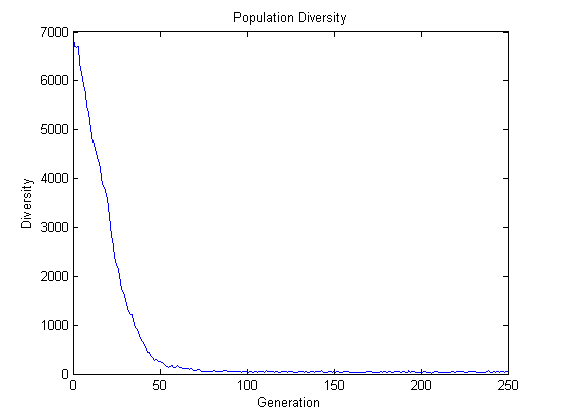
\includegraphics[scale=0.6]{BlendDiversity.png}
	 % \caption{\label{fig:blendDiversity} Picture showing the diversity grapth for blend crossover.}
 % \end{figure}

\begin{table}[h]
\scalebox{0.8}{
\begin{tabular}{|l|l|l|l|}
\hline
\multicolumn{4}{|l|}{Blend Fitness, getting fit without workout! Different Mutation Strategies}                              \\ \hline
Mutate Proportional & Mutate Decay = None & Mutate Decay = Linear & Mutate Decay = Exponential \\ \hline
True                & 2.1                 & 1.8                   & 2.9                        \\ \hline
True                & 2.7                 & 2.7                   & 13.7                       \\ \hline
True                & 2.5                 & 1.9                   & 1.6                        \\ \hline
True                & 2.1                 & 2.7                   & 2.8                        \\ \hline
True                & 2.3                 & 12.7                  & 2.7                        \\ \hline
False               & 1.7                 & 2.0                   & 2.6                        \\ \hline
False               & 12.7                & 2.9                   & 1.7                        \\ \hline
False               & 2.3                 & 2.2                   & 2.9                        \\ \hline
False               & 2.4                 & 2.8                   & 3.0                        \\ \hline
False               & 2.5                 & 1.9                   & 2.1                        \\ \hline
\end{tabular}}
\caption{Comparing Mutation Strategies}
\label{table:mutationStrategies}
\end{table}
 
\subsection*{Question 12}
\emph{Which (if any) of the dynamic mutation probability strategies
improved the performance of the algorithm? What difference do you observe in the results?}

\textbf{Answer:} As we can see in Table \ref{table:mutationStrategies} we can't really see any difference between the different mutation strategies. Since the values are few and that the blend crossover earlier experienced some random high fitness values we can't really draw any conclusions from these values except that all strategies seems equally good. 

We will choose to continue the experiments with Linear Mutation strategy and no proportional mutations. 

\subsection*{Question 13}
\emph{Describe the effect (if any) comparative selection has on population diversity and convergence.} 

\textbf{Answer:} Every run with comparative selection we achieve a fitness value of 0 with the selected parameters. Blend crossover, Linear Mutation and no proportional mutation. Compared with Arithmetic crossover the results seems to be slightly better but nearly as good as with the Blend crossover. 

\subsection*{Question 14}
\emph{What was the fitness value and position of the best solution you
were able to locate? Report the parameter settings you used to generate that solution.} 

\textbf{Answer:} As mentioned in Question 13 we get fitness 0 every experiment we have conducted. The parameters are: Crossover function = blend, Pressure = 2, Generation = 250, Mutate probability = 0.003, Mutate Decay = Linear, Mutate Proportional = False, Population Size = 200, Comparative = True, Elitist = True, Selection = Proportional and Selection Pressure = 2.

\subsection*{Question 15}
\emph{Try using GAsolver to find the minimum for the 100 dimensional Ackley's function, using the same parameters as the last question. How
well does it perform now? Can you improve the performance?} 

\textbf{Answer:} It only performed decent with a fitness between 1.5-2.5. We discovered that we could increase the performance by simply increasing the number of generations it could run. 1000 generations is sufficient to find the optimal solution to a 100 dimensional Ackley's function.

\section*{Task 3: Particle Swarm Optimization}

\subsection*{Question 16}
\emph{What happens to the maximum velocity of the swarm over time
when using velocity clamping? How does the maximum velocity compare with
the theoretical velocity limit (the red line at the top of the velocity plot)?} 

\textbf{Answer:} The max velocity of the swarm over time flattens to a quite stable value below the theoretical velocity limit. 

\begin{table}[h]
\scalebox{1.0}{
\begin{tabular}{|l|l|l|l|l|}
\hline
\multicolumn{5}{|c|}{Magical constant optimization} \\ \hline
Velocity Limit  & $c_1$  & $c_2$& $w$   & Fitness \\ \hline
1               & 2     & 2     & 1       & 3.06    \\ \hline
1               & 1.49  & 1.49  & 0.7968  & 0.00    \\ \hline
500             & 1.49  & 1.49  & 0.7968  & 0.09    \\ \hline
500             & 1.49  & 1.49  &[0.9;0.4]& 0.00    \\ \hline
\end{tabular}}
\caption{Testing different magical constants}
\label{table:magicConstants}
\end{table}

\subsection*{Question 17}
\emph{What values for $w$, $c_1$ and $c_2$ worked best on this problem? How close did this swarm come to locating the global optimum?} 

\textbf{Answer:} As seen in Table \ref{table:magicConstants} the magical values of $c_1 = c_2 = 1.49$ and $w = 0.7968$ seem to strongly improve the best found fitness value. It found the global optimum. 

\subsection*{Question 18}
\emph{Was velocity clamping still necessary to prevent swarm explosion, or were you able to find a combination of values that kept the swarm together?} 

\textbf{Answer:} Now it's not necessary since solution with velocity limit 500 found a solution even though it took more time.

\subsection*{Question 19}
\emph{What was the best combination of decaying inertia weights, and social and cognitive coefficients? What was the best fitness value you found using that combination?}

\textbf{Answer:} As seen in the last row in Table \ref{table:magicConstants} it found the global optimum. However this combination found the global optimum in fewer generations than previous experiments. 

\subsection*{Question 20}
\emph{What is the equation for the value of the constriction coefficient
in terms of $\Phi$?}

\textbf{Answer:}

\begin{align*}
\chi = \frac{2\kappa}{|2-\phi-\sqrt{\phi(\phi-4)}|}
\end{align*}


\subsection*{Question 21}
\emph{Consider the constriction equation with $\Phi_1 = 4, \Phi_2 = 2$. What is
the constriction coefficient for these values? What values of $w, c_1$ and
$c_2$ would we have to use in (2) in order to implement constriction with these
values?}

\textbf{Answer:}

With $c_1 = c_2 = \phi = \phi_1 + \phi_2 = 4 + 2 = 6$ we get:
\begin{align*}
\chi = \frac{2\kappa}{|2-6-\sqrt{6(6-4)}|} = (2-\sqrt{3})\kappa
\end{align*}

And to implement constriction, we should use $w = \chi, c_1 =
\frac{\phi_1}{\chi}, c_2 = \frac{\phi_2}{\chi}$

\subsection*{Question 22}
\emph{Describe the behavior of the swarm when using constriction.
Does it locate the global optimum? How quickly does it converge?}

\textbf{Answer:}

\section*{Task 4: Global Trajectory Optimisation}

\subsection*{Question 23}
\emph{Before trying to solve this problem, make a hypothesis. Consider what little you know about the problem. Now, make an educated guess: what is one choice for setting up either GA or PSO which you think might lead to better performance on this problem? For example, you could hypothesize that a particular crossover operation will be more effective than the others, or that higher values of social attraction will improve PSO performance. Your choice needs to be something you can test in matlab , and should be more than simply changing the number of iterations or population size. Briefly explain why you
think that your choice might make a difference on this problem. (Note that there isn’t a right or wrong answer here.)}

\textbf{Answer:}

\section*{4.1 GA}

\subsection*{Question 24}
\emph{Describe your final GA setup, in enough detail that your experiment can be replicated (the output of ga show parameters can be useful here). Which settings seemed to have the most effect on your final results?}

\textbf{Answer:}

\subsection*{Question 25}
\emph{What was the best solution you were able to locate? Be sure to
include both the fitness value, and the full 22-dimensional vector representing
the solution. How long did it take to run the solver?}

\textbf{Answer:}

\section*{4.2 PSO}

\subsection*{Question 26}
\emph{Describe your final PSO setup, in enough detail that your experiment can be replicated (the output of \texttt{psooptimset} can be useful here). Which settings seemed to have the most effect on your final results?}

\textbf{Answer:}

\subsection*{Question 27}
\emph{What was the best solution you were able to locate? Be sure to
include both the fitness value, and the full 22-dimensional vector representing the solution. How long did it take to run the solver?}

\textbf{Answer:}

\section*{4.3 Testing Your Hypothesis}

\subsection*{Question 28}
\emph{Describe your experimental setup, and summarise your results.
Did the experiment support or contradict your hypothesis? Be persuasive. (Note: plots are persuasive.)}

\textbf{Answer:}

\section*{Task 5: Wrapping up}

\subsection*{Question 29}
\emph{How well did today's lab help to reinforce concepts from the
lectures? Is there a specific concept that the lab has helped to clarify for you? Is there a concept from the relevant lectures that should have been covered more?}

\textbf{Answer:}

\subsection*{Question 30}
\emph{If you attended it, then how helpful did you find today's lab
session? What could have been improved?}

\textbf{Answer:}


\end{document}
